\begin{mainquestion}{fgenloading}{Function Generators and Oscilloscope Probes} As you may have seen in Lab 1, the function generators in the
laboratory can be simply configured with an output magnitude $V_m$.  Internally, this value is used to model a voltage source with amplitude $V_{\mathrm{gen}}$ which is placed in series with a $\qty{50}{\ohm}$ source resistance; this is illustrated in the accompanying circuit diagram.
By default, the function generator ``assumes'' it will be connected to a matched load; that is, a load $R_L$ whose resistance matches that of the source---namely
$\qty{50}{\ohm}$.


\begin{center}
    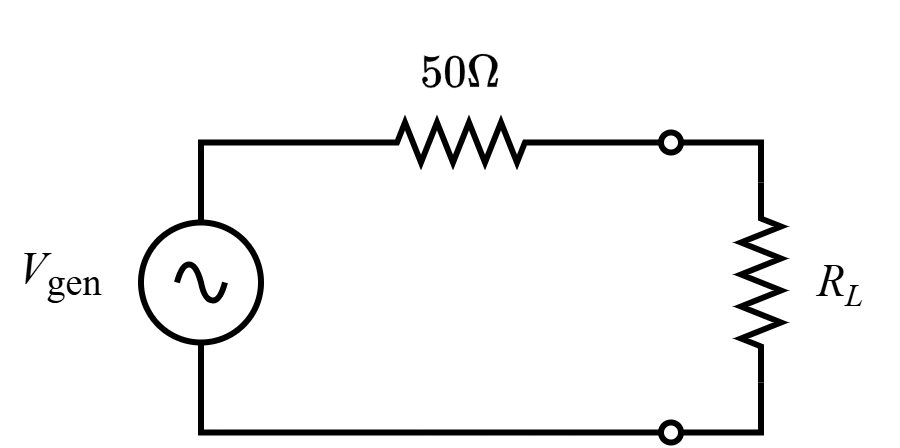
\includegraphics[width=4.7in]{circuit.png}
\end{center}

\begin{partquestion}{mag}{In a matched-load scenario, if the output (load) voltage is configured to have an amplitude of $\qty{10}{\volt}$, what is the actual value of $V_\mathrm{gen}$ set by the function generator?}
\begin{answer}
Because the function generator is expecting a matching load of $\qty{50}{\ohm}$, it expects
to deliver what is configured, $\qty{10}{\volt}$, at the load. Since
\[
V_L = V_{\mathrm{gen}}\frac{R_L}{\qty{50}{\ohm} + R_L},
\]
we have
\[
V_{\mathrm{gen}}
=V_L\frac{\qty{50}{\ohm}+R_L}{R_L}
=(\qty{10}{\volt})\frac{\qty{50}{\ohm}+\qty{50}{\ohm}}{\qty{50}{\ohm}}
=\qty{20}{\volt}.
\]
\end{answer}
\end{partquestion}
\begin{partquestion}{power}{What percentage of the power in the circuit is dissipated in the load in this scenario?}
\begin{answer}
For a periodic signal with amplitude $V_m$, the power dissipated in a resistor is always proportional to $\frac{V_m^2}{R_L}$.  
\[
P_L=\alpha\frac{V_L^2}{R_L}
=\alpha\frac{(\qty{10}{\volt})^2}{\qty{50}{\ohm}}
=2\alpha\,\mathrm{W}.
\]
The total power dissipated is
\[
P_{\mathrm{total}}
=\alpha\frac{V_{\mathrm{gen}}^2}{\qty{50}{\ohm}+R_L}
=\alpha\frac{(\qty{20}{\volt})^2}{\qty{100}{\ohm}}
=4\alpha\,\mathrm{W},
\]
so the percentage dissipated in the load is
\[
\frac{P_L}{P_{\mathrm{total}}}
=\frac{2\alpha\,\mathrm{W}}{4\alpha\,\mathrm{W}}
=0.5=50\%.
\]
\end{answer}
\end{partquestion}
\begin{partquestion}{mag2}{Now assume the load $R_L$ is not $\qty{50}{\ohm}$ but a $1\,\mathrm{M}\Omega$ oscilloscope channel input. If the function generator remains configured as in part (\cref{prob:fgenloading:mag}), what is the amplitude of the voltage that will be displayed on the oscilloscope?}
\begin{answer}
The internally generated source voltage remains $V_{\mathrm{gen}}=\qty{20}{\volt}$, but now
\[
V_L
=V_{\mathrm{gen}}\frac{1\,\mathrm{M}\Omega}
{\qty{50}{\ohm}+1\,\mathrm{M}\Omega}
\approx V_{\mathrm{gen}}
=\qty{20}{\volt}.
\]
\end{answer}
\end{partquestion}
\begin{partquestion}{voltadj}{How should the function-generator voltage be adjusted to provide the expected voltage across the load?}
\begin{answer}
We would need to drop the function-generator setting such that $V_m = \qty{5}{\volt}$, requiring that
\[
V_{\mathrm{gen}}=V_L=\qty{10}{\volt}.
\]
\end{answer}
\end{partquestion}
\begin{partquestion}{power2}{What percentage of the power in the circuit is now dissipated in the load?}
\begin{answer}
The power dissipated in the load is
\[
P_L=\alpha\frac{V_L^2}{R_L}
=\alpha\frac{(\qty{10}{\volt})^2}{1\,\mathrm{M}\Omega}
=0.1\alpha\,\mathrm{mW}.
\]
The total power dissipated is
\[
P_{\mathrm{total}}
=\alpha\frac{V_{\mathrm{gen}}^2}{\qty{50}{\ohm}+R_L}
=\alpha\frac{(\qty{10}{\volt})^2}{\qty{50}{\ohm}+1\,\mathrm{M}\Omega}
\approx 0.1\alpha\,\mathrm{mW},
\]
so the percentage dissipated in the load is approximately
\[
\frac{0.1\alpha\,\mathrm{mW}}{0.1\alpha\,\mathrm{mW}}
=1.0=100\%.
\]
\end{answer}
\end{partquestion}
\begin{partquestion}{sourcer}{What is the approximate source resistance of a $20{:}1$
oscilloscope probe?}
\begin{answer}
We require the voltage provided to the oscilloscope to be $1/20$ of the actual measured
voltage:
\[
\frac{V_{\mathrm{scope}}}{V_{\mathrm{probe}}}
=\frac{R_{\mathrm{scope}}}{R_{\mathrm{probe}}+R_{\mathrm{scope}}}
=\frac{1}{20}.
\]
Since the oscilloscope has a $1\,\mathrm{M}\Omega$ input,
\[
\frac{1\,\mathrm{M}\Omega}{R_{\mathrm{probe}}+1\,\mathrm{M}\Omega}
=\frac{1}{20},
\]
and therefore
\[
R_{\mathrm{probe}}=19\,\mathrm{M}\Omega.
\]
\end{answer}
\end{partquestion}
\begin{partquestion}{secondscope}{Now imagine you took such a probe attached (and properly configured)
to a second identical oscilloscope and measured the voltage of the load $R_L$ coming into
the first oscilloscope still configured as in part (\cref{prob:fgenloading:voltadj}). What is the voltage level seen by
the second oscilloscope? What is the voltage level displayed by the second oscilloscope?}
\begin{answer}
The voltage seen by the second oscilloscope is $1/20$ of the actual voltage, which was
determined to be $\qty{10}{\volt}$. Thus,
\[
V_{\mathrm{seen}}=\qty{0.5}{\volt}.
\]
Because the second oscilloscope is properly configured with the $20{:}1$ probe attenuation
factor, it compensates for this factor of 20 and displays
\[
V_{\mathrm{displayed}}=\qty{10}{\volt}.
\]
\end{answer}
\end{partquestion}

\end{mainquestion}


